\documentclass[11pt,letterpaper]{article}

\usepackage{showlabels}
\usepackage{fullpage}
\usepackage{pslatex}
%\usepackage{latexsym}
\usepackage[english]{babel}
\usepackage[utf8]{inputenc}
\usepackage{amsmath}
\usepackage{bm}
%\usepackage{tikz}
\usepackage{xcolor}
\usepackage{url}
%\usepackage[colorinlistoftodos]{todonotes}
\usepackage{rotating}
\usepackage{natbib}
\usepackage{amssymb}
\usepackage{lingmacros}


%\usepackage{latexsym}
\usepackage[english]{babel}
\usepackage[utf8]{inputenc}
\usepackage{bm}
\usepackage{graphicx}
%\usepackage{tikz}
\usepackage{xcolor}
\usepackage{url}
%\usepackage[colorinlistoftodos]{todonotes}
\usepackage{rotating}
\usepackage{multirow}

\usepackage{hyperref}

\usepackage{tikz-dependency}
\usepackage{changepage}
\usepackage{longtable}
\usepackage{pdfpages} 

\newcommand{\R}[0]{\mathbb{R}}
\newcommand{\Prob}[0]{\mathbb{P}}
\newcommand{\Ff}[0]{\mathcal{F}}

\usepackage{multirow}

\newcommand{\soft}[1]{}
\newcommand{\nopreview}[1]{}
\newcommand\comment[1]{{\color{red}#1}}
\newcommand\mhahn[1]{{\color{red}(#1)}}
\newcommand\note[1]{{\color{red}(#1)}}
\newcommand\jd[1]{{\color{red}(#1)}}
\newcommand\rljf[1]{{\color{red}(#1)}}
\newcommand{\key}[1]{\textbf{#1}}

\DeclareMathOperator*{\argmax}{arg\,max}
\DeclareMathOperator*{\argmin}{arg\,min}
\DeclareMathOperator{\E}{\mathop{\mathbb{E}}}


\newcommand{\infdiv}{D\infdivx}
\newcommand{\future}{\overrightarrow{X}}
\newcommand{\past}{\overleftarrow{X}}
\newcommand{\finitefuture}{\stackrel{\rightarrow \scriptscriptstyle{M}}{X}}
\newcommand{\finitepast}{\stackrel{\scriptscriptstyle{M}\leftarrow}{X}}%_{-M\dots -1}}



\usepackage{amsthm}

\newcommand{\thetad}[0]{{\theta_d}}
\newcommand{\thetal}[0]{{\theta_{LM}}}

\newcounter{theorem}
\newtheorem{proposition}[theorem]{Proposition}
\newtheorem{thm}[theorem]{Theorem}
\newtheorem{corollary}[theorem]{Corollary}
\newtheorem{question}[theorem]{Question}
\newtheorem{example}[theorem]{Example}
\newtheorem{defin}[theorem]{Definition}
\newtheorem{definition}[theorem]{Definition}
\newtheorem{lemma}[theorem]{Lemma}


%\usepackage{linguex}
%\newcommand{\key}[1]{\textbf{#1}}



\renewcommand{\thefigure}{S\arabic{figure}}
\renewcommand{\thetable}{S\arabic{table}}
\renewcommand{\thesection}{S\arabic{section}}

\newcommand{\utterance}{\mathcal{U}}
\newcommand{\tree}{\mathcal{T}}



\usepackage{siunitx}



\usepackage{longtable}



\frenchspacing
%\def\baselinestretch{0.975}

%\emnlpfinalcopy
%\def\emnlppaperid{496}

\title{Supplement: Theoretical Limitations of Self-Attention in Neural Sequence Models}
\author{Michael Hahn}
\date{\today}

\begin{document}

\maketitle

Here I am providing two supplements to the published TACL paper:
First, a more formal writeup of the hard attention proof. This has benefited a lot from discussions with Gail Weiss and Will Merrill.
Second, I am providing a missing detail in the soft attention proof (thanks for Navin Goyal and Satwik Bhattamishra for spotting this).


\section{Results for Hard Attention}

\begin{thm}\label{thm:hardmax-main}
Let any hard attention transformer be given, and let $C \in (0,1)$.
Then there is a restriction $\rho$ and an integer $c > 0$ such that 
$$|\{i \leq n: \rho_n(i) = *\}| \geq Cn$$
(for all sufficiently large $n$) and such that the function computed by the transformer on the restricted input depends only on $\leq c$ inputs, independent of input length $n$.
\end{thm}


\begin{defin}[$c$-Transformer]
Let $c$ be a positive integer. A $c$-transformer is one in which the layer-0 activations $y_j^{(0)}$ depend on the embeddings not just at one position $j$, but are a function of the embeddings at $\leq c$ input positions:
\begin{equation}
    y_j^{(0)} = f^{inp}_{n,j}((v_{i_1^{j,n}}, p_{i_1^{j,n}}), \dots, (v_{i_c^{j,n}}, p_{i_c^{j,n}} ))
\end{equation}
for some indices ${i_s^{j,n}} \in \{1, \dots, n\}$ ($s = 1, \dots, c$).
\end{defin}

\begin{defin}
We say $\rho' \succ \rho$ if, whenever $\rho'_n(i) = *$, then $\rho_n(i) = *$.

We write $\rho T$ for the function resulting from applying $\rho$ to $T$.

We write $\rho\Sigma^*$ for the set of inputs compatible with $\rho$.
\end{defin}


With this technical notion, we show that we can reduce layers, iteratively removing the lowest layer until no self-attention layer is left:

\begin{lemma}[Depth Reduction Lemma]\label{lemma:depth-red}
Given a $c$-transformer $T$ with $L$ layers, and some restriction $\rho$ such that
\begin{equation}
|\{i \leq n: \rho_n(i) = *\}| \geq Cn
\end{equation}
($C \in (0,1]$)
for all sufficiently large $n$.
Choose any $C' < C$.

Then there is a restriction $\rho' \succ \rho$ 
such that
\begin{equation}
|\{i \leq n: \rho'_n(i) = *\}| \geq C'n
\end{equation}
for all sufficiently large $n$, 
and such that there is a $( c\cdot(2^ckH+1))$-transformer $T'$ with $L-1$ layers, for some integer $k$ (depending on $C'$), where $H \geq 1$ is the number of attention heads at each layer and position, such that $\rho'T = \rho' T'$.
\end{lemma}
The lemma implies Theorem~\ref{thm:hardmax-main}:
\begin{proof}[Proof of Theorem~\ref{thm:hardmax-main}]
The output of the transformer is determined by the last activation $y_{n}^{(L)}$.
Apply the Depth Reduction Lemma iteratively, choosing the constants $C'$ in the lemma appropriately, until only the zero-th layer remains.
Then, after applying the resulting restriction, the final activation $y_{n}^{(L)}$ is now computed by $y_{n}^{(0)}$, which is determined by a bounded number of input bits.
\end{proof}



\subsection{Proving the Depth Reduction Lemma}
In this section, we will prove the Depth Reduction Lemma.
We construct the restrictions $\rho'_n$ separately for each $n$, on the basis of the given restriction $\rho_n$.
In this process, we will only \emph{restrict additional bits}, that is, the only case in which $\rho_n'(i)$ can be different from $\rho_n(i)$ is that $\rho_n'(i)$ may be $0$ or $1$ where $\rho_n(i)$ was $*$.
The construction proceeds in three stages $\rho_n^{(1)}$, $\rho_n^{(2)}$, and $\rho_n^{(3)} = \rho_n'$, which all may restrict additional bits.
At the end, we verify that the conclusion of the Depth Reduction Lemma is satisfied for the resulting restriction $\rho_n'$.

Throughout the proof, we will need a few parameters independent of $n$: First, we need an integer $k$ that has to be sufficiently large for the proof to succeed, and will be fixed later in the proof.
Second, we need parameters $\eta \in (0, \frac{1}{2})$, $q \in (0,1)$ and $\delta > 0$; they can be chosen as follows:

\begin{defin}\label{def:constants}
Choose $\eta \in (0,\frac{1}{2})$ small, $q \in (0,1)$, and $\delta >0$ (such that $(1+\delta)q \in (0,1)$) in such a way as to achieve
\begin{equation}
    (1-2\eta)\cdot (1-(1+\delta)q) = C'/C
\end{equation}
A possible choice to satisfy this is $(1+\delta)q = \frac{1}{2}$, $2\eta = 1-2C'/C$.
\end{defin}


\begin{lemma}[Stage 1]\label{lemma:stage1}
There is $N$ and a restriction $\rho^{(1)} \succ \rho$ such that 
\begin{enumerate}
    \item each $\rho^{(1)}$-free input bit serves as an input to at most $\leq \frac{1}{\eta} c/C$ many different layer-0 heads, when applying $\rho^{(1)}_n$.
    \item For $n > N$, 
    \begin{equation}
        \#\{i \leq n: \rho^{(1)}_n(i) = *\} \geq (1-\eta) C n
    \end{equation}
\end{enumerate}
\end{lemma}
\begin{proof}
Assume the number of input bits feeding into more than $\frac{1}{\eta} c/C$ different layer-0 activations is $\geq \eta Cn$.
Then the number of pairs of input bits and depending layer-0 activations is $>\eta Cn \cdot \frac{1}{\eta} c/C = nc$.
But there are at most $nc$ such pairs, because there are $n$ layer-0 activations, each of which depends on $\leq c$ inputs.
So the number of input bits with $> \frac{1}{\eta} c/C$ depending layer-0 heads is $\leq \eta Cn$.
We can obtain $\rho^{(1)}_n$ from $\rho_n$ by restricting these input bits to some fixed value in $\{0, 1\}$ (it doesn't matter which one), and the set $\{i \leq n: \rho^{(1)}_n(i) = *\}$ still has at least $(1-\eta) C n$ elements, for all sufficiently large $n$.
\end{proof}


We write $(h,i)$ for a layer-1 attention head $h$ ($h=1,\dots, H$) at position $i$ ($i=1, \dots, n$).
Let $V_\rho(i)$ denote the possible values of $y^{(0)}_i$.
As $y^{(0)}_i$ depends on $\leq c$ input bits, we have:
\begin{equation}
|V_\rho(i)| \leq 2^c
\end{equation}

\begin{defin}
For a restriction $\rho$, a head $(h,i)$, a value $z \in V_\rho(i)$,  and each position $j \in \{1, \dots, n\}$, set
\begin{equation}\label{eq:max-att}
A_{((h,i),z),j,\rho} := \max_{x_1\dots x_n \in \rho\Sigma^n\ :\ y^{(0)}_i=z} f^{att}_{1,h}(z, y^{(0)}_j)
\end{equation}
For each value $z \in V_\rho(i)$, we rank the positions $\{1, \dots, n\}$ downwards by this value, obtaining a sequence (in the case of ties, we resolve as we do when computing hard attention)
\begin{equation}
J_{((h,i,z), \rho} := \left(j_1^{(z)}, \dots, j_n^{(z)}\right)    
\end{equation}
For each $((h,i),z)$, obtain the sequence
\begin{equation}
1 \leq i_1^{(h,i,z,\rho)} < i_2^{(h,i,z,\rho)} < \dots < i_{L}^{(h,i,z,\rho)} \leq n
\end{equation}
of those indices $j$ such that there is some $\rho$-free input $x_q$ that feeds into the activation at $j$ and no activation and $j' < j$.
\end{defin}


%\begin{lemma}
%Take a layer-1 head $((h,i),z)$ and an input $x_j$. 
%Assume $\rho(j) = *$ and $x_j$ appears as an input to some $j_{i_s^{(h,i,z,\rho)}}$ where $s \leq k$.
%Then $((h,i),z)$ $(k,\rho)$-depends on input $x_j$.
%\end{lemma}
%\emph{The converse does not hold in general.}
%\begin{proof}
%From the construction of the sequence.
%\end{proof}


\begin{defin}[Satisfaction]
Let $\sigma$ be a restriction, and $k \in \mathbb{N}$, and assume  $z \in V_\sigma(i)$.
We say that a pair $((i,h),z)$ is $(k,\sigma)$-\key{satisfied} if %one of the layer-0 activations $y^{(0)}_{j_{s}^{(h,i,z,\sigma)}}$ ($s \in \{1, \dots k\}$) is fixed by $\sigma$ to a specific value.
its function value depends on at most $\leq ck$ many input bits when applying $\rho$.
\end{defin}

\begin{lemma}[Satisfaction and Dependency]\label{lemma:satis-dep}
If $((h,i),z)$ is $(k,\sigma)$-unsatisfied, then the sequence
\begin{equation}
\left(   i_s^{(h,i,z,\rho)} : s=1, \dots, L   \right)
\end{equation}
has length $L$ at least $\geq $k.
\end{lemma}

\begin{proof}
Assume some of the layer-0 heads it $(k,\rho)$-depends on.
The higher-ranked layer-0 heads can only have a total of $\leq ck$ inputs, contradiction.
\end{proof}


%\begin{defin}[Satisfaction]
%Let $\sigma$ be a restriction, and assume  $z \in V_\sigma(i)$.
%We say that a pair $((i,h),z)$ is $(k,\sigma)$-select-\key{satisfied} if
%\begin{enumerate}
%    \item Either $L \leq k$, OR
%    \item one of the layer-0 activations $y^{(0)}_{j_{i_s}^{(h,i,z,\sigma)}}$ ($s \in \{1, \dots k\}$) is fixed by $\sigma$ to a specific value.  (SELECT-SATISFIED)
    %the value achieving the maximum attention value $A_{((h,i),z), i_s^{(z)}, \sigma}$ (said differently, the maximum in the definition is trivial).
%\end{enumerate}
%\end{defin}

\begin{lemma}[Preservation of Satisfaction]\label{lemma:satisfied-preserved}
Let $\sigma$ be a restriction, and $k \in \mathbb{N}$.
If $((i,h),z)$ is $\sigma$-satisfied, and $\sigma' \succ \sigma$, then $((i,h),z)$ is also $\sigma'$-satisfied.
\end{lemma}

\begin{proof}
Immediate.
\end{proof}



\begin{defin}
An unsatisfied tuple $((h,i),z)$ $(k,\rho)$-\textbf{depends} on some input $x_i$ if $\rho(i) = *$ and $x_i$ appears as an input to some $j_r^{(h,i,z,\rho)}$ for $r \leq i_k^{(h,i,z,\rho)}$.
\end{defin}

\begin{defin}
An unsatisfied tuple $((h,i),z)$ $(k,\rho)$-\textbf{depends} on some layer-0 head $j$ if $j = j^{(h,i,z,\rho)}_s$ for some $s \leq i_k$.
\end{defin}

\begin{lemma}\label{lemma:depend-bits-count}
 $((h,i),z)$ $(k,\rho)$-{depends} on $x_i$ iff $x_i$ appears as an input to some $j^{(h,i,z,\rho)}_{i_s}$ ($s \leq i_k$).
 
  Hence, $((h,i),z)$ $(k,\rho)$-{depends} on at most $\leq ck$ input bits.
\end{lemma}
\begin{proof}
From the definitions.
\end{proof}

\begin{defin}
Two unsatisfied tuples $((h,i),z)$, $((h',i'),z')$  are $(k,\rho)$-\textbf{neighbors} if some $j_{i_s^{(h,i,z,\rho)}}$ for one and $j_{i_{s'}^{(h',i',z',\rho)}}$ for the other both $(k,\rho)$-depend on some input bit $x_l$.
\end{defin}


\begin{lemma}
Let $\rho$ be a restriction, and $k \in \mathbb{N}$.
Assume the layer-0 head at position $j$ has more than $2^c kH$ many $(k,\rho)$-depending  $(k,\rho)$-unsatisfied tuples $((h,i),z)$.
Then there is a restriction $\rho' \succ \rho$, restricting only $\leq c$ additional inputs, such that at least $kH$ many $(k,\rho)$-unsatisfied tuples $((h,i),z)$ become $(k,\rho')$-satisfied.
\end{lemma}

\begin{proof}
Let $\rho$ be a restriction, and $k \in \mathbb{N}$.
Assume the layer-0 head at position $j$ has more than $2^c kH$ many $(k,\rho)$-depending  $(k,\rho)$-unsatisfied tuples $((h,i),z)$.
For each $(k,\rho)$-depending $(k,\rho)$-unsatisfied tuple $((h,i),z)$, collect the value $q'$ of $y_j^{(0)}$ ($q' \in V_\rho(j)$) resulting in $A_{((h,i),z),j,\rho}$.
There are $> 2^c kH$ such tuples, but only $2^c$ possible values $q'$. So one value $q$ of them must occur $> kH$ times, by the Pigeonhole Principle.
Thus, this $q \in V_\rho(j)$ is such that
\begin{equation}
    f^{att}_{1,h}(z, q) = A_{((h,i),z),j,\rho}
\end{equation}
for at least $> kH$ many of these $(k,\rho)$-depending tuples $((h,i),z)$.

For such a tuple $((h,i),z)$, $j$ now blocks attention on any lower-ranked elements of the ranking.
The higher-ranked elements of the ranking can only depend on a total of $\leq ck$ input bits by Lemma~\ref{lemma:depend-bits-count}.
\end{proof}




\begin{defin}[Sequence of Restrictions]
Define a (finite or infinite) sequence of restrictions $\rho^{(1)} = \sigma_1 \prec \sigma_2 \prec \dots$ as follows:
\begin{enumerate}
\item $\sigma_1 := \rho^{(1)}$
\item Let $\sigma_i$ be given ($i \geq 1$). If a layer-0 head has more than $2^c kH$ many $(k,\sigma_i)$-depending $(k,\sigma_i)$--unsatisfied tuples $((h,i),z)$, fix $\leq c$ input bits to make $\geq kH$ tuples satisfied, using the preceding lemma, obtaining $\sigma_{i+1}$.
Otherwise, terminate the procedure.
\end{enumerate}
\end{defin}

\begin{lemma}\label{lemma:termination}
There are $K, N$ such that for all $k > K$, $n > N$, this procedure terminates with $\rho'_n \succ \rho^{(1)}_n$ such that
\begin{enumerate}
    \item We have
\begin{equation}
    \# \{i \leq n: \rho'_n(i) = *\} \geq (1-2\eta) C n
\end{equation}
\item No layer-0 head has more than $2^c kH$ many $(k,\rho')$-depending $(k,\rho')$-unsatisfied tuples $((h,i),z)$.
\end{enumerate}
\end{lemma}

\begin{proof}
Due to Lemma~\ref{lemma:satisfied-preserved}, this procedure can be iterated at most until each tuple $((h,i),z)$ is $(k,\sigma_i)$-satisfied, that is, at most
\begin{equation}
\frac{2^c H n}{kH} = \frac{2^c n}{k}
\end{equation}
times.
Let $U_n$ be the number of times this procedure is iterated ($U_n \leq \frac{2^c n}{k}$).
At the end, for $n > N$,
\begin{equation}
\#\left\{i \leq n: (\sigma_U)(i) = *\right\} \geq (1-\eta) C n - cU_n \geq \left((1-\eta) C  - \frac{2^c c}{k}\right) n
\end{equation}
By choosing $k$ so large that $\frac{2^c c}{k} \leq \eta C$, we find that
\begin{equation}
    \# \{i \leq n: (\sigma_U)_n(i) = *\} \geq (1-2\eta) C n
\end{equation}
for every $n > N$.
For the second claim, if this were not the case, the procedure would not have terminated at $\rho'_n$.
\end{proof}

\begin{corollary}[Stage 2]\label{cor:stage-2}
There is $K, N$ such that, for each $k > K$, there is a restriction $\rho^{(2,k)} \succ \rho^{(1)}$ such that

\begin{enumerate}
\item $\# \{i \leq n: \rho^{(2,k)}_n(i) = *\} \geq (1-2\eta) C n$ for each $n > N$
\item Every $(k,\rho^{(2,k)})$-unsatisfied $((h,i),z)$ has at most $f \leq \frac{2^{2c}}{\eta}c^2k^2H/C$ many $(k,\rho^{(2,k)})$-unsatisfied $(k,\rho^{(2,k)})$-neighbors.
\end{enumerate}
\end{corollary}

\begin{proof}
Let $\rho^{(2,k)}$ be as given by Lemma~\ref{lemma:termination}.
The first assertion is immediate from that lemma.
For the second assertion, by that lemma, each layer-0 head has at most $\leq 2^c kH$ many $(k,\rho^{(2)})$-depending $(k,\rho^{(2)})$-unsatisfied tuples $((h,i),z)$.
Using Lemma~\ref{lemma:stage1} and Lemma~\ref{lemma:depend-bits-count}, each input bit has at most $\leq \frac{2^c}{\eta}kcH/C$ many $(k,\rho^{(2)})$-depending $(k,\rho^{(2)})$-unsatisfied tuples.
On the other hand, a tuple $((h,i),z)$ can $(k,\rho^{(2)})$-depend on  $\leq k c$ inputs by Lemma~\ref{lemma:depend-bits-count}.
Multiplying these two bounds gives $\leq \frac{2^{2c}}{\eta}k^2c^2H/C$.
\end{proof}

%We will write $\rho^{(2)}$ for some such restriction, keeping $k$ implicitly as an argument. I.e., more formally, we should be writing $\rho^{(2,k)}$, but we'll suppress that argument.

In order to construct the third and final restriction $\rho^{(3)}_n$, we apply the ``probabilistic method'': We define a probability distribution over restrictions $\rho^{(3)}_n$, and show that the probability assigned to restrictions of the type we require is strictly greater than zero, showing that such a restriction exists.

\begin{defin}
Let $k > K$.
For each input length $n$, define the distribution over restrictions $\rho_n^{(3,k)} \succ \rho_n^{(2,k)}$ that independently assigns to each input position $i \in \{1, \dots, n\}$ the symbol $1$ or $0$ with probability $q/2$ each ($q \in (0,1)$ from Definition~\ref{def:constants}), and $*$ with probability $1-q$.
On those input bits where $\rho_n^{(2,k)}(i) \neq *$, we restrict this random restriction to agree with $\rho_n^{(2,k)}(i)$.
\end{defin}
%By definition, $\rho_n^{(3,k)} \succ\rho_n^{(2,k)}(i)$ for every restriction $\rho_n^{(3,k)}$ with nonzero probability.

\begin{defin}
Let $k > K$, and consider a $(k, \rho^{(2,k)})$-unsatisfied tuple $((h,i),z)$.
By Lemma~\ref{lemma:satis-dep}, the sequence
\begin{equation}
\left(   y_{j_{i_s^{(z)}}}^{(0)} : s=1, \dots, L   \right)
\end{equation}
has length at least $\geq $k.

Define $X_{i,h,k}^{(z)}$ to be the event that, for this tuple, none of the $k$ layer-0 head it depends on ($s = 1, \dots, k$) is fixed by $\rho^{(3,k)}$ to the value
\begin{equation}
    \arg_{q \in V_{\rho^{(2,k)}}(j_{i_s^{(h,i,z,\rho^{(2)})}})} \max f^{att}_{1,h}(z, q)
\end{equation}
(or any element of the argmax, if multiple values achieve this attention weight).

Define $X_{0,k}$ to be the event that more than $(1+\delta)q$ of the input bits that $\rho_n^{(2,k)}$ maps to $*$ are set to $0/1$ by $\rho_n^{(3,k)}$ (where $\delta \in (0,1)$ was fixed in Definition~\ref{def:constants}).
\end{defin}



Our goal will be to show that a nonzero amount of probability mass is assigned to restrictions $\rho_n'$ avoiding all events.
We start by individually bounding the probability of each of these events.

\begin{lemma}[$X_{0,k}$ is unlikely]
For any $n > N, k > K$:
\begin{equation}
\Prob(X_{0,k}) \leq    \exp\left(-\frac{\delta^2q(1-2\eta)Cn}{3}\right)
\end{equation}
\end{lemma}

\begin{proof}
Since $\rho_n^{(2,k)}$ had $\geq (1-2\eta)Cn$ unrestricted input bits for $n > N$, this follows by a Chernoff bound~\cite[Theorem 4.4]{mitzenmacherprobability}.
\end{proof}

Second, we show that the probability of $X_{i,h,k}^{(z)}$ ($i=1,2,\dots, n$, $h=1, \dots, H$) decays exponentially in $k$.

\begin{lemma}[$X_{i,h,k}^{(z)}$ is unlikely]
If $((h,i),z)$ is $(k,\rho)$-unsatisfied, then
\begin{equation}
\Prob(X_{i,h,k}^{(z)}) \leq \left(1-(q/2)^c\right)^{\frac{k}{\frac{1}{\eta}c^2/C}}
\end{equation}
for each $i=1,2,\dots, n$ and $h=1, \dots, H$.
\end{lemma}
\begin{proof}
Let $Y_{i,h,z,k}^t$ ($t=1,\dots,k$) be the event that the layer-0 activation $y_{j_{i_t^{(h,i,z,\rho^{(2)})}}}^{(0)}$ is not fixed by $\rho^{(3,k)}$ to
\begin{equation}
    \arg_{q \in V_{\rho^{(2,k)}}(j_{i_t^{(h,i,z,\rho^{(2)})}})} \max f^{att}_{1,h}(z, q)
\end{equation}
%the highest attention weight, for the given attention head $((h,i),z)$.
Note that
\begin{equation}
    X_{i,h}^{(z)} = \bigcap_{t=1}^k Y_{i,h}^t
\end{equation}
We have 
\begin{equation}
    \Prob(Y_{i,h}^s) \leq 1-(q/2)^c \in (0,1)
\end{equation} 
Any $Y_{i,h,z}^s$ can be statistically dependent on at most 
\begin{equation}
c \cdot \frac{1}{\eta}c/C = \frac{1}{\eta}c^2/C    
\end{equation}
other events $Y_{i,h,z}^{s'}$, because each $\rho^{(2,k)}$-free input bit serves as an input to at most
\begin{equation}
    \frac{1}{\eta} c/C
\end{equation}
layer-0 heads (Lemma~\ref{lemma:stage1}).
Therefore, there is a set of
\begin{equation}
    \geq \frac{k}{\frac{1}{\eta}c^2/C}
\end{equation} independent events among these.
Call these $Y_{i,h}^{t_1}, \dots, Y_{i,h}^{\frac{k}{\frac{1}{\eta}c^2/C}}$.
Then 
\begin{equation}
    X_{i,h}^{(z)} \subseteq \bigcap_{s=1}^{\frac{k}{\frac{1}{\eta}c^2/C}} Y_{i,h}^{t_s}
\end{equation}
and thus
\begin{equation}
\Prob(X_{i,h}^{(z)}) \leq \prod_{s=1}^{\frac{k}{\frac{1}{\eta}c^2/C}} \Prob(Y_{i,h}^{t_s}) \leq \left(1-(q/2)^c\right)^{\frac{k}{\frac{1}{\eta}c^2/C}}
\end{equation}
for each $i=1,2,\dots, n$ and $h=1, \dots, H$.
\end{proof}



\begin{lemma}\label{lemma:lovasz}
There are $N, K$ such that, for each $n >N$, $k > K$, the probability of avoiding all events
\begin{equation}
\{X_{0,k}\} \cup \{X_{i,h,k}^{(z)} : ((h,i),z) \text{ is } (k,\rho^{(2,k)})\text{-unsatisfied}\}
\end{equation}
is strictly greater than zero.
\end{lemma}

\begin{proof}
We apply the Lov{\'a}sz Local Lemma \cite[Theorem 6.17]{mitzenmacherprobability}.
Each event $X_{i,h,k}^{(z)}$ is statistically independent of the set 
\begin{equation}
    \left\{X_{(j,h',k)}^{(z')} : (k,\rho^{(2,k)})\text{-unsatisfied tuples } {(j,h',z')} \text{ and } {(i,h,z)} \text{ are not $(k, \rho^{(2,k)})$-neighbors}\right\}
\end{equation}
The complement of this set has cardinality 
\begin{equation}
    \leq f= \frac{2^{2c}}{\eta}c^2k^2H/C
\end{equation}
as concluded in Corollary~\ref{cor:stage-2}.
Set $A:=\frac{1}{k^2}$, $B:=\frac{1}{2}$.
The number of events $X_{i,h}^{(z)}$ is bounded by $2^c H n$.
By the Lov{\'a}sz Local Lemma, it is sufficient show the following: %, assuming $f \leq $:
\begin{align}\label{eq:lovasz-1}
&\Prob(X_{i,h}^{(z)}) \leq A(1-B)(1-A)^{f} \\ \label{eq:lovasz-2}
&\Prob(X_0)  \leq B (1-A)^{2^cHn}
\end{align}
The Lov{\'a}sz Local Lemma then guarantees that there is some input restriction $\rho^{(3)}_n$ that avoids all events $\{X_0\} \cup \{X_{i,h,k}^{(z)} : i, h, z\}$.
For~(\ref{eq:lovasz-1}), we need
\begin{align}\label{eq:x1-ineq}
    D &\leq A^{1/k}(1-B)^{1/k}(1-A)^{f/k} 
\end{align}
where $D =  \left(1-(q/2)^c\right)^{\frac{1}{\frac{1}{\eta}c^2/C}} \in (0,1)$.
For the first term on the right, 
\begin{align*}
\lim_{k\rightarrow \infty} A^{1/k} = \lim_{k\rightarrow \infty} \exp\left(-\log(k^2) / k\right) = 1
\end{align*}
Also, $\lim_{k\rightarrow \infty} (1-A)^{f/k}$ equals
\begin{align*}
\lim_{k\rightarrow \infty} \left(1-\frac{1}{k^2}\right)^{\frac{2^{2c}}{\eta}c^2kH/C} = \lim_{k\rightarrow \infty} \left(1-\frac{E^2}{k^2}\right)^{k} = 1
\end{align*}
for $E := \frac{2^{2c}}{\eta}c^2H/C$. So, if we choose $k$ large enough (independently of $n$), the RHS of (\ref{eq:x1-ineq}) can be made arbitrarily close to $1$, in particular, greater than $D$.
In order to also satisfy~(\ref{eq:lovasz-2}), we need
\begin{align*}
\exp\left(-\delta^2q(1-2\eta)C/3\right)  \leq B^{1/n} (1-A)^{2^c H}
\end{align*}
which holds for $n$, $k$ large enough (again, choosing $k$ independent of $n$). 
\end{proof}


\begin{corollary}
There are $K, N$ such that for $n > N$, $k > K$, for any $\rho^{(3,k)}_n$ provided by Lemma~\ref{lemma:lovasz}, we have 
\begin{equation*}
|\{i \leq n: \rho^{(3,k)}_n(i) = *\}|\geq C' n
\end{equation*}
\end{corollary}

\begin{proof}
We have 
\begin{equation*}
|\{i \leq n: \rho^{(3,k)}_n(i) = *\}|\geq (1-2\eta)\cdot (1-(1+\delta)q) C n
\end{equation*}
for all sufficiently large $n$.
The claim follows from the choices in Definition~\ref{def:constants}.
\end{proof}


\begin{proof}[Proof of the Depth Reduction Lemma]
After applying $\rho^{(3,k)}_n$, every layer-1 head $b_{j,1,h}$ depends at most on 
\begin{enumerate}
    \item the $c$ input bits feeding into $y_j^{(0)}$, and
    \item for each $h=1, \dots, H$, $z \in V_{\rho^{(3,k)}}(j) \subseteq V_{\rho^{(2,k)}}(j)$ such that $((h,j),z)$ is  $(k,\rho^{(2,k)})$-\textbf{satisfied}, at most $\leq ck$ input bits by the definition of ``satisfied''.
    \item for each $h=1, \dots, H$, $z \in V_{\rho^{(3,k)}}(j) \subseteq V_{\rho^{(2,k)}}(j)$ such that $((h,j),z)$ is  $(k,\rho^{(2,k)})$-\textbf{unsatisfied}, the input bits that the tuple $k$-depends on, of which there are at most $\leq ck$ by Lemma~\ref{lemma:depend-bits-count}. (Stated differently, every tuple is $(k,\rho^{(3,k)})$-satisfied.)
\end{enumerate}
Thus, each layer-1 activation $y_j^{(1)}$ only depends on $\leq c\cdot (2^ckH+1)$ input bits.

We can thus remove layer 0, convert layer-1 activations $y_j^{(1)}$ into layer-0 activations $y_j^{(0)}$, and obtain a $(c\cdot(2^ckH+1))$-transformer performing the same computation as before when $\rho^{(3)}$ is applied.
\end{proof}


\section{Missing Detail in Soft Attention Proof}

In the proof of Lemma 5 on Page 11, the inequality at the end of the first column has the form
\begin{equation}
	\|b - b'\| < \sum  a_w \| y_w -y'_w\|
\end{equation}
A term is missing: the RHS should be of the form
\begin{equation}
	\|b - b'\| < \sum  a_w \| y_w -y'_w\| + \sum |a_w – a’_w| y’_w
\end{equation}
The missing term is also small under the assumptions used in the paper.

First, $y'_w$ is bounded because $f^{att}$ and $f^{act}$ are Lipschitz functions, and the positional embeddings are assumed to be bounded. These assumptions are used in the k=0 step of the proof of Lemma 5, and they are necessary for the proof to work.

Second, $\sum |a_w – a’_w|$ is also in O(1/n). The next page contains a calculation for this claim.


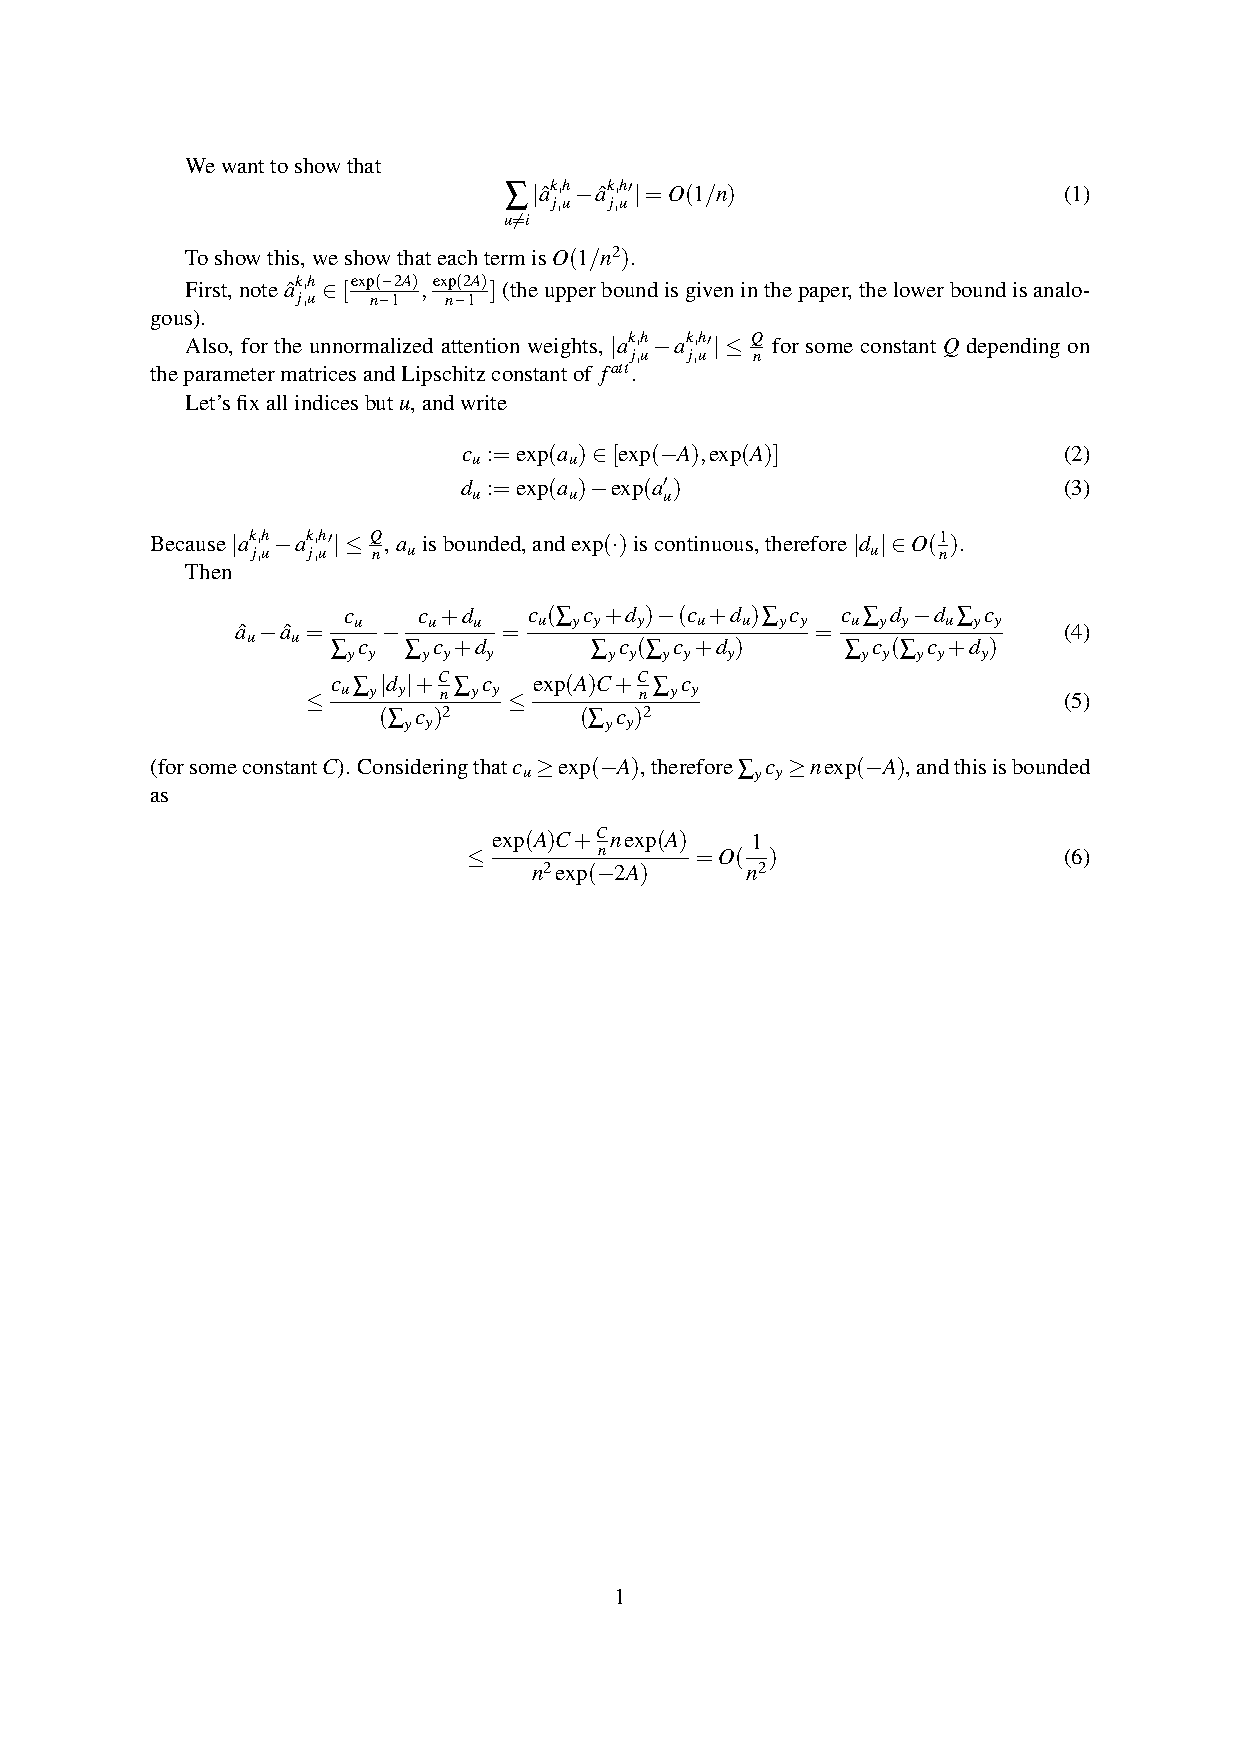
\includepdf[pages={1}]{attention_bound.pdf}


\section*{Acknowledgments}
Thanks for Gail Weiss, Will Merrill, Navin Goyal, and Satwik Bhattamishra for helpful discussion about the original paper.


\bibliographystyle{apalike}
\bibliography{literature}

\end{document}

